\documentclass[a4paper,11pt]{article}
\usepackage[hidelinks, colorlinks=true, urlcolor=blue, linkcolor=black, citecolor=blue]{hyperref}
\usepackage[english]{babel}
\usepackage{unicode-math}
\usepackage{xunicode}
\usepackage{url}
\usepackage{cite}
\usepackage{graphicx}
\usepackage[justification=centering, labelfont=bf]{caption}
\usepackage{float}
\usepackage{pgfgantt}
\usepackage{marvosym}
\usepackage{siunitx}
\usepackage{multirow}
\usepackage[nottoc,numbib]{tocbibind}
\usepackage{indentfirst}
\usepackage{afterpage}
\usepackage{minted}
\usepackage{tabularx}
\usepackage{tikz}
\usetikzlibrary{arrows,positioning}
\setlength{\parindent}{24pt}
\usepackage{fontspec}
\usepackage{parskip}
\usepackage{fancyhdr}
\usepackage{titlesec}

\defaultfontfeatures{Scale=MatchLowercase}
\setmainfont[Ligatures=TeX,
BoldFont=texgyrepagella-bold.otf,
BoldItalicFont=texgyrepagella-bolditalic.otf,
ItalicFont=texgyrepagella-italic.otf]{texgyrepagella-regular.otf}
\setsansfont[Ligatures=TeX,
BoldFont=lmsans10-bold.otf,
BoldItalicFont=lmsans10-boldoblique.otf,
ItalicFont=lmsans10-oblique.otf]{lmsans10-regular.otf}
\setmonofont[BoldFont=lmmonolt10-bold.otf,
BoldItalicFont=lmmonolt10-boldoblique.otf,
ItalicFont=lmmono10-italic.otf,
SlantedFont=lmmonoslant10-regular.otf]{lmmono10-regular.otf}
\setmathfont{texgyrepagella-math.otf}
\setmathfont[range={\mathcal,\mathbfcal},StylisticSet=1]{xits-math.otf}
\setlength{\parindent}{24pt}
\setcounter{secnumdepth}{5}
\setcounter{tocdepth}{1}


 
\pagestyle{fancy}
\fancyhf{}
\fancyhead[LE,RO]{Héctor Ramón}
\fancyhead[RE,LO]{\leftmark}
\fancyfoot[RE]{Final degree project}
\fancyfoot[LO]{\emph{Web platform for multiplayer programming games}}
\fancyfoot[LE,RO]{\thepage}

\renewcommand{\footrulewidth}{0.5pt}
\setlength{\marginparwidth}{0pt}
\setlength{\parskip}{0.8em}


\titleformat{\chapter}{\normalfont\bfseries}{\Huge\thechapter}{20pt}{\Huge}
\newcommand*{\fullref}[1]{\hyperref[{#1}]{\autoref*{#1} \nameref*{#1}}}

\setcounter{secnumdepth}{5}
\setcounter{tocdepth}{2}
\begin{document}
\begin{titlepage}
\begin{center}
\textsc{\Large Degree Final Project}
\\[1.5cm]
\rule{\linewidth}{0.5mm}
\\[0.4cm]
{\huge
\bfseries
Web platform for massive multiplayer programming games
\\[0.4cm]
}
\rule{\linewidth}{0.5mm}
\\[0.3cm]
{\bfseries
Monitoring report
}
\\[2.5cm]
\begin{center}
\large
Héctor Ramón Jiménez
\end{center}
Directed by Jordi Petit Silvestre
\vfill
{\large
Facultat d'Informàtica de Barcelona
}
\\[0.5cm]
{\large
\today
}
\end{center}
\end{titlepage}
\clearpage
\tableofcontents
\clearpage
\section{Introduction}
\subsection{Playing games while programming}
In 1961, \textbf{Victor Vyssotsky}, a mathematician and computer scientist working at Bell Labs, had an idea. He devised
a computer game, but not a traditional one where the player inputs the different actions from a controller to play it.
No. He wanted to create a game that it could only be played by writing a \textbf{computer program}. And so, along with \textbf{Robert
Morris Sr.} and \textbf{Doug McIlroy}, they created \textbf{Darwin} \cite{darwin}: the first programming game.

A \textbf{programming game} is a computer game where the player does not directly interact with the game. Instead, the
player writes a \textbf{computer program} that plays the game. These \textbf{computer programs} are usually called \textbf{artifficial
intelligences} (\textbf{AI}s) because they try to make intelligent decisions to win the game.

\textbf{Darwin} consisted of two or more small programs, written by the players, that were loaded in memory. The main goal
of the game was to spread copies of your own program and find and kill the copies of other players. The game was only
played for a few weeks before Morris developed an ultimate program, as no-one managed to produce anything that could
defeat it.

Since then, many other programming games have been created \cite{pg}. Some of them are even commercial games, like
\textbf{SpaceChem} \cite{spacechem}.
\subsection{Playing with other people}
With the arrival of the \textbf{Internet} and the \textbf{W}orld \textbf{W}ide \textbf{W}eb, there was nothing stopping people from
developing \textbf{multiplayer programming games}.

A \textbf{multiplayer programming game} is a \textbf{programming game} where multiple players compete with each other to win the
game. Thus, the game becomes a challenge where strategy and programming skills make the difference.

Web platforms have been created that allow players to compete with each other easily. For example, \textbf{Robot Game}
\cite{robotgame} is a website where anyone can upload an \textbf{AI} written in \texttt{Python} and compete with other people.
\subsection{Playing while learning}
Writing \textbf{AI}s can be a really fun and rewarding experience because the game allows the players to see how their
\textbf{algorithms work visually}, while competition motivates them to \textbf{learn and improve}.

It is not a surprise, then, that programming games are being used in schools to teach students different programming
techniques. For instance, an \textbf{AI programming challenge} is held every semester in the \textbf{Barcelona School of
Informatics} (\textbf{FIB}) where students enrolled in the subject \textbf{Data Structures and Algorithms} (\textbf{EDA}) \cite{eda}
compete with each other in a multiplayer programming game using the \textbf{Jutge} platform \cite{jutge}.

However, current multiplayer programming games feature \textbf{short matches} with a \textbf{small number of players}. There
is no way to perform a challenge with a considerable amount of students playing at the same time. Therefore, multiple
matches are necessary to decide who wrote the best program.
\subsection{A new era: playing with everyone at the same time}
It is time to take multiplayer programming games to the next level, featuring \textbf{huge worlds}, \textbf{long matches} and
a \textbf{massive amount of players in real-time}. Games where the player will feel attached to the match, where constant
\textbf{evolution} and adaptation matters, where your program plays with everyone at the same time. It is time to create
\textbf{massive multiplayer programming games} (\textbf{MMPG}s).
\clearpage
\vspace*{\fill}
\begin{center}
\emph{This document details the current status of the project and the changes made to the original planning.}
\end{center}
\vfill
\clearpage
\section{Component status}
\label{components}
\subsection{Engine}
The \texttt{MMPG} \textbf{engine} is a library that implements basic features needed by any \texttt{MMPG}. The \textbf{engine} exposes a set
of classes that can be used and extended to build the logic of the game.

Its source code is available here: \url{https://github.com/mmpg/engine}
\subsubsection{Architecture}
The runtime of an \texttt{}MMPG\texttt{} \textbf{engine} consists of 3 types of processes:
\begin{description}
\item[Master process]
It represents the \textbf{game-world server}. The master process listens to requests coming from
players and updates the game world accordingly. There is only \textbf{one master process per runtime}.
\item[Worker process]
It represents a \textbf{pool of players}. A worker process \textbf{executes} a set of players and
  \textbf{manages} them. There can be \textbf{multiple workers per runtime}.
\item[Player process]
It represents a \textbf{player program}. A player process \textbf{reads} the game world from the
  \textbf{master process} and \textbf{performs requests} to \textbf{change} the game world.
\end{description}
Processes comunicate with each other using \textbf{low-latency sockets}. Thus, different workers can be executed
in different machines to achieve better performance.

\autoref{engine_arch} shows the hierarchy of an engine runtime with $N$ workers and $M = \sum_{i=0}^{N} M_i$ players.
\begin{figure}[!h]
\noindent\resizebox{\textwidth}{!}{
\begin{tikzpicture}[->,>=stealth',shorten >=1pt,auto,node distance=0.8cm,
    main node/.style={thick,circle,draw,minimum width=2.5cm}]

    \node[main node] (1) {master};

	\node[auto=false] (2) [below=of 1]{\ldots};
    \node[auto=false] (21) [left=of 2]{};
    \node[auto=false] (23) [left=of 21]{};
    \node[auto=false] (22) [right=of 2]{};
    \node[auto=false] (24) [right=of 22]{};

    \node[main node] (3) [left=of 23]{worker$_1$};
    \node[main node] (4) [right=of 24]{worker$_N$};

    \node[auto=false] (5) [below=of 3]{\ldots};
    \node[main node] (6) [left=of 5]{player$_{1,1}$};
    \node[main node] (7) [right=of 5]{player$_{1,{M_1}}$};

    \node[auto=false] (8) [below=of 4]{\ldots};
    \node[main node] (9) [left=of 8]{player$_{N,1}$};
    \node[main node] (10) [right=of 8]{player$_{N,{M_N}}$};


    \path (1) edge (3);
    \path (1) edge (4);

    \path (3) edge (6);
    \path (3) edge (7);

    \path (4) edge (9);
    \path (4) edge (10);
\end{tikzpicture}

}
\caption{Hierarchy of engine processes}
\label{engine_arch}
\end{figure}
\subsubsection{Current features}
\begin{description}
\item[AI hot-swapping]
Players can change their programs during a match.
\item[Log system]
Every event that occurs in the engine is logged properly. This allows players to replay and
  watch the past of a match.
\item[Event notification]
Events are notified to subscribers through a \texttt{PUB/SUB} socket connection.
\item[Decoupled architecture]
The current architecture makes scaling easy. Each worker can be executed in a
  different machine.
\item[API]
The engine listens to requests made through a \texttt{REQ/REP} socket connection. Other applications can
  easily connect to the engine and interact with it.
\item[Game abstraction]
A set of abstract classes defines the behaviour that any \texttt{MMPG} needs to implement.
  Mostly, this behaviour includes the \textbf{AI public interface}, \textbf{game actions}, and \textbf{world generation and
  serialization}.
\end{description}
\subsubsection{Pending features}
\begin{description}
\item[Security]
Programs need to be executed in an isolated environment.
\item[Configuration]
Ports used in socket connections and worker addresses should be configurable.
\end{description}
\subsubsection{Implementation details}
\paragraph{Programming language}
\hfill
\\[0.2cm]
\indent
The \textbf{engine} needs to be \textbf{fast}, as the game logic will be built on top of it, and it also needs to access
\textbf{low-level} operative system operations, so it can limit how player programs are executed. Hence, \textbf{\texttt{C}++} is the
programming language chosen to implement it, mainly because its \textbf{efficiency} and the \textbf{\texttt{}C\texttt{ POSIX API}}, which allows
to talk directly to \textbf{\texttt{UNIX}-based operative systems}.
\paragraph{Inter-process communication}
\hfill
\\[0.2cm]
\indent
As it was explained previously, the \textbf{engine} features a decoupled architecture. Different processes are
executed and communicate with each other using \textbf{sockets}. However, implementing inter-process communication from
scratch would be a real challenge by itself, and it is not the subject of this project. This is where \textbf{\texttt{ZeroMQ}} comes
in.

\textbf{\texttt{ZeroMQ}} is an embeddable networking library that implements \textbf{low-latency socket communication}. It manages
\textbf{low-level} communication, while providing a flexible and easy-to-use interface. \textbf{\texttt{ZeroMQ}} has bindings available
for the most well-known programming languages.

The \textbf{engine} uses \textbf{\texttt{ZeroMQ}} for all the inter-process communication. As a consequence, the architecture becomes
decoupled. For instance, a \textbf{player process} could be programmed in \textbf{any programming language}, as it
only performs requests to the master process. Thus, it would be \textbf{relatively easy} to allow players to develop
\textbf{AI}s using \textbf{different programming languages}.
\paragraph{Game logic abstraction}
\hfill
\\[0.2cm]
\indent
The \textbf{engine} exposes a set of \textbf{abstract classes} to build game logic on top of it:
\begin{description}
\item[\texttt{AI}]
Defines the interface that any \texttt{MMPG} AI needs to implement: a \texttt{play} method. Games can extend
  this class to define \textbf{\texttt{AI API}s} that players can use to write their programs.
\item[\texttt{World}]
Represents a game world. Games need to extend this class and implement methods to
  \textbf{generate}, \textbf{serialize} and \textbf{update} the world.
\item[\texttt{Action}]
Represents an action that an \textbf{AI} can perform. Normally, these actions try to \textbf{update}
  the game world.
\end{description}
On the other hand, the \textbf{engine} also provides two \textbf{fully-implemented classes} to run \textbf{master and player
processes}. As \autoref{world_injection} shows, a game world needs to be injected to run these processes.

The \textbf{worker process} is \textbf{independent of the game logic} and it can be built \textbf{directly from the library}.
\begin{figure}[!h]
\inputminted[linenos,fontsize=\small,frame=lines,framesep=2mm]{c++}{code/master.cpp}
\caption{Injecting a game world to the master process}
\label{world_injection}
\end{figure}
\subsection{API}
The \textbf{\texttt{API}} component exposes \textbf{\texttt{HTTP}} endpoints that allow to interact with an underlying \textbf{engine}. It
usually handles requests from the game viewer.

The \textbf{\texttt{API}} component is developed using the \textbf{\texttt{Go}} programming language \cite{golang}. \textbf{Go}
is \textbf{simple}, \textbf{fast}, \textbf{easy-to-deploy} and includes \textbf{native} libraries to build \texttt{REST API}s.

It source code is available here: \url{https://github.com/mmpg/api}
\subsubsection{Current endpoints}
\begin{tabularx}{\textwidth}{l | l | X}
\textbf{URI} & \textbf{Method} & \textbf{Description}\\
\hline
\texttt{/auth} & \texttt{GET} & Validates an authentication token and returns a new one.\\
\texttt{/auth} & \texttt{POST} & Validates the given user credentials and returns an authentication token.\\
\texttt{/log} & \texttt{GET} & Returns the log file of the given \textbf{time}.\\
\texttt{/events} & \texttt{GET} & Upgrades the HTTP request to a WebSocket subscription of engine events.\\
\texttt{/player} & \texttt{POST} & Deploys the uploaded file as the player of the authencated user.\\
\end{tabularx}
\subsubsection{Pending endpoints}
\begin{tabularx}{\textwidth}{l | l | X}
\textbf{URI} & \textbf{Method} & \textbf{Description}\\
\hline
\texttt{/world} & \texttt{GET} & Returns the current state of the world.\\
\end{tabularx}
\\[0.2cm]
\indent
This endpoint might be useful to reduce the amount of information in the events, as the \textbf{static} part of
the game world would not need to be included anymore.
\subsection{Client}
The \textbf{client} component is a \textbf{JavaScript} library that implements a set of useful classes to communicate with
an \textbf{\texttt{MMPG} \texttt{API}} and implement \textbf{game viewers}.

Its source code is available here: \url{https://github.com/mmpg/client}
\subsubsection{Current classes}
\begin{description}
\item[\texttt{Client}]
Allows to perform requests to any \textbf{\texttt{MMPG} \texttt{API}}. Most of its methods perform an \texttt{HTTP} request
  and return a JavaScript \textbf{promise}.
\item[\texttt{EventStream}]
Represents a stream of game events. It delegates the event handling to its \textbf{subscriber}.
\item[\texttt{LiveSubscriber}]
\textbf{Buffers} 2 seconds of events and then starts \textbf{consuming them}.
\item[\texttt{PlaybackSubscriber}]
Reads a \textbf{log} of events from the \texttt{API} and consumes them. When the number of
  events reaches a minimum, it requests the next log to the \texttt{API}.
\item[\texttt{Webtoken}]
Represents a \textbf{\texttt{JSON} Webtoken} \cite{jwt}. It is used to manage authentication tokens.
\item[\texttt{GameLoop}]
Implements a \textbf{consistent game loop}, calling a callback function and passing the time
  between calls as the first argument.
\end{description}
\subsection{Space Wars}
\textbf{Space Wars} will be the first game using the \texttt{MMPG} platform. It is inspired by \textbf{Galcon} \cite{galcon}
and \textbf{Planet Wars} \cite{planet_wars}.
\subsubsection{Logic}
...
\subsubsection{Viewer}
...
\section{Planning}
\subsection{Time management}
\autoref{gantt_original} shows the original time planning, while \autoref{gantt_current} shows the final time
planning.

\begin{figure}[!h]
\makebox[\textwidth]{
\noindent\resizebox{300pt}{!}{
\begin{ganttchart}[hgrid, vgrid]{1}{25}
\gantttitle{2015}{20}
\gantttitle{2016}{5}
\\
\gantttitle{September}{5}
\gantttitle{October}{5}
\gantttitle{November}{5}
\gantttitle{December}{5}
\gantttitle{January}{5}
\\
\ganttbar{Project management}{3}{8}
\\
\ganttbar{Analysis and design}{4}{5}
\\
\ganttbar{Game engine}{6}{10}
\\
\ganttbar{Real-time notifier}{11}{13}
\\
\ganttbar{Notifier subscriber}{14}{15}
\\
\ganttbar{Control panel}{16}{17}
\\
\ganttbar{Game example - logic}{11}{18}
\\
\ganttbar{Game example - viewer}{16}{20}
\\
\ganttbar{Testing and polishing}{21}{22}
\\
\ganttbar{Project memory}{11}{23}
\\
\ganttbar{Oral presentation}{24}{24}
\ganttlink{elem1}{elem2}
\ganttlink{elem2}{elem3}
\ganttlink{elem3}{elem4}
\ganttlink{elem4}{elem5}
\ganttlink{elem2}{elem6}
\ganttlink{elem4}{elem7}
\ganttlink{elem6}{elem8}
\ganttlink{elem7}{elem8}
\ganttlink{elem2}{elem9}
\ganttlink{elem9}{elem10}
\end{ganttchart}
}
}
\caption{Original time planning}
\label{gantt_original}
\end{figure}
\begin{figure}[!h]
\makebox[\textwidth]{
\noindent\resizebox{300pt}{!}{
\begin{ganttchart}[hgrid, vgrid]{1}{25}
\gantttitle{2015}{20}
\gantttitle{2016}{5}
\\
\gantttitle{September}{5}
\gantttitle{October}{5}
\gantttitle{November}{5}
\gantttitle{December}{5}
\gantttitle{January}{5}
\\
\ganttbar{Project management}{3}{11}
\\
\ganttbar{Analysis and design}{6}{7}
\\
\ganttbar{Engine}{9}{15}
\\
\ganttbar{API}{9}{13}
\\
\ganttbar{Client}{9}{13}
\\
\ganttbar{Space Wars - logic}{16}{19}
\\
\ganttbar{Space Wars - viewer}{16}{20}
\\
\ganttbar{Testing and polishing}{21}{22}
\\
\ganttbar{Project memory}{16}{23}
\\
\ganttbar{Oral presentation}{24}{24}
\ganttlink{elem1}{elem2}
\ganttlink{elem1}{elem3}
\ganttlink{elem1}{elem4}
\ganttlink{elem2}{elem5}
\ganttlink{elem3}{elem6}
\ganttlink{elem4}{elem6}
\ganttlink{elem5}{elem7}
\ganttlink{elem6}{elem7}
\ganttlink{elem8}{elem9}
\end{ganttchart}
}
}
\caption{Final time planning}
\label{gantt_current}
\end{figure}
The first change to notice is that some components have been \textbf{renamed}. Also, the control panel has been
\textbf{integrated} inside the game viewer, as described in \autoref{components}.

The most important change, though, is that the components \textbf{engine}, \textbf{API}, and \textbf{client} have been developed
in parallel in order to perform \textbf{continuous integration} so there is always a working prototype of the project.
This change is described with more detail in \autoref{methodology}.
\clearpage
\subsection{Dedication}
\begin{figure}[!h]
\makebox[\textwidth]{
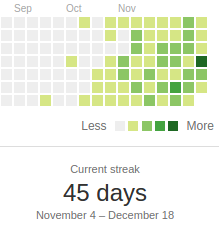
\includegraphics[scale=0.5]{images/dedication.png}
}
\caption{GitHub contributions to the \texttt{MMPG} project}
\label{dedication}
\end{figure}
\clearpage
\section{Methodology}
\label{methodology}
CI
\clearpage
\bibliographystyle{plain}
\bibliography{references}
\end{document}
